\documentclass[border=4pt]{standalone}
\usepackage{fontspec}
\usepackage{amsmath}
\usepackage{unicode-math}
\setmainfont{Latin Modern Roman}
\setmathfont{Latin Modern Math}
\usepackage{pgfplots}
\usepackage{pgfplotstable}
\pgfplotsset{compat=1.18}
\usepackage{tkz-euclide}
\usetikzlibrary{arrows.meta,calc,angles,quotes,patterns,3d,backgrounds}
\definecolor{ink}{HTML}{123428}
\definecolor{asy}{HTML}{475569}
\definecolor{mint}{HTML}{86e0bd}
\tikzset{asym/.style={asy, line width=0.9pt, dash pattern=on 5pt off 3.5pt},
         guide/.style={gray!70, line width=0.6pt, densely dotted},
         dot/.style={circle, inner sep=0pt, minimum size=5pt, draw=white, line width=0.5pt},
         odot/.style={circle, inner sep=0pt, minimum size=5.5pt, fill=white, line width=1pt},
         lab/.style={font=\footnotesize, inner sep=1.5pt, text=ink}}
\begin{document}
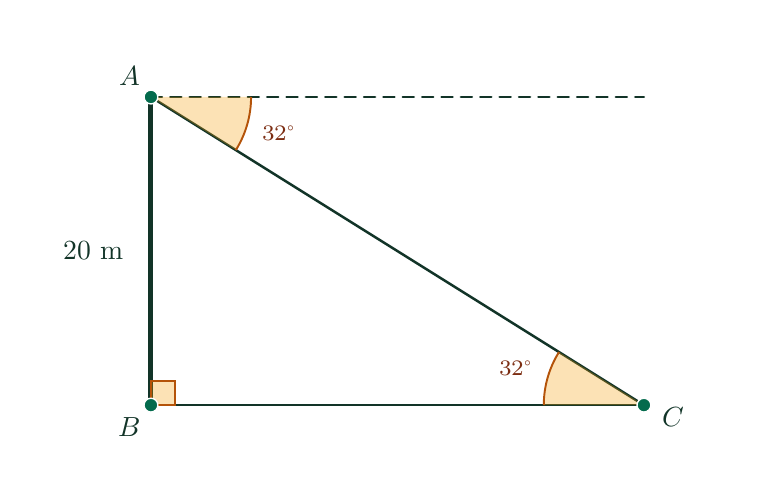
\begin{tikzpicture}[x=0.9783cm, y=0.9783cm]
\tkzDefPoint(0,4){A}
\tkzDefPoint(0,0){B}
\tkzDefPoint(6.4,0){C}
\tkzDefPoint(6.4,4){H}
\begin{scope}
\clip (-1.6,-0.9) rectangle (7.6,4.9);
\tkzDrawSegment[draw=ink, line width=1.80pt](B,A)
\tkzDrawSegment[draw=ink, line width=0.90pt](B,C)
\tkzDrawSegment[draw=ink, line width=0.90pt](A,C)
\tkzDrawSegment[draw=ink, line width=0.90pt, dash pattern=on 4pt off 3pt](A,H)
\end{scope}
\tkzMarkRightAngle[size=0.31, draw={rgb,255:red,180;green,83;blue,9}, line width=0.7pt, fill={rgb,255:red,245;green,158;blue,11}, fill opacity=0.3](C,B,A)
\tkzFillAngle[size=1.3, fill={rgb,255:red,245;green,158;blue,11}, fill opacity=0.3](C,A,H)
\tkzMarkAngle[size=1.3, draw={rgb,255:red,180;green,83;blue,9}, line width=0.7pt, mark=none](C,A,H)
\tkzLabelAngle[pos=1.729, text={rgb,255:red,124;green,45;blue,18}, font=\footnotesize](C,A,H){$32^\circ$}
\tkzFillAngle[size=1.3, fill={rgb,255:red,245;green,158;blue,11}, fill opacity=0.3](A,C,B)
\tkzMarkAngle[size=1.3, draw={rgb,255:red,180;green,83;blue,9}, line width=0.7pt, mark=none](A,C,B)
\tkzLabelAngle[pos=1.729, text={rgb,255:red,124;green,45;blue,18}, font=\footnotesize](A,C,B){$32^\circ$}
\node[dot, fill={rgb,255:red,4;green,107;blue,77}] at (A) {};
\node[dot, fill={rgb,255:red,4;green,107;blue,77}] at (B) {};
\node[dot, fill={rgb,255:red,4;green,107;blue,77}] at (C) {};
\node[lab, font=\normalsize] at (-0.75,2) {$20\text{ m}$};
\node[lab, font=\normalsize, anchor=center, xshift=-7.78pt, yshift=7.78pt] at (0,4) {$A$};
\node[lab, font=\normalsize, anchor=center, xshift=-7.78pt, yshift=-7.78pt] at (0,0) {$B$};
\node[lab, font=\normalsize, anchor=center, xshift=10.16pt, yshift=-4.21pt] at (6.4,0) {$C$};
\end{tikzpicture}
\end{document}
